\documentclass{article}

\usepackage{ctex}
\usepackage{amsmath}
\usepackage{amssymb}
\usepackage{amsthm}
\usepackage{amsfonts}
\usepackage{graphicx}
\usepackage{float}

\usepackage[a4paper, left=1in, right=1in, top=1in, bottom=1in]{geometry}

\title{\textbf{数学与现代音乐}}
\author{曹陈都 3230104276}
\date{\today}

\begin{document}

\maketitle

\begin{abstract}
\label{abstract}
本文探究了现代音乐在分析与创作中蕴含的数学规律。通过集合论、抽象代数、Fourier 分析等非传统的数学音乐方法,我们得以更深入地理解音乐的结构和形式。通过特定的算法与生成模型,我们还可以将数学方法用于实际的音乐创作,实现数学与音乐的深刻交融。
\end{abstract}

\section{引言}
\label{sec:introduction}
数学自古以来就与音乐有着密切的联系。早在古希腊时期,毕达哥拉斯就发现了音高与弦长之间的比例关系:当琴弦弦长减半时,音高就会提高一个八度\cite{math_history_2017}。两根按特定比例调好的琴弦发出的声音将会是“协和”的,例如八度音程、五度音程等,这些比例关系可以用整数比来表示。对于毕达哥拉斯及其学派的古希腊人来说,数学与音乐存在着如此天然的和谐关系。

毕达哥拉斯在此基础上还提出了“五度相生律(Pythagorean Tuning)”,这是最早而最为广泛应用的律制之一。其以一个基础音为起点,通过的频率比为3:2的五度音程连续相生,从而推导出音阶中的其他音。但五度相生循环12次之后,得到的音高与起始音的八度音存在了一个较小的偏差,这个偏差被称为“毕式音差”,在特定情况下其影响了音乐的和谐性。

律制经过长时间的发展,最终演变成了“十二平均律(Equal Temperament)”这一较为完备的形式。最早发现十二平均律的是我国明代的学者朱载堉,而将其在音乐创作中发扬光大的是“音乐之父”巴赫。十二平均律将一个八度音程分为12个等分音程,使得每个音程的频率比为$\sqrt[12]{2}$,从而消除了毕式音差。这一律制的广泛应用使得音乐创作和演奏变得更加灵活和多样化\cite{math_art_2021}。

\section{音高集合论}
\label{sec:pitch_set_theory}
20世纪初期,在“调性危机”的时代背景下,以勋伯格(Arnold Schoenberg)为首的一批音乐家开始了“无调性”音乐的创作。“无调性”音乐并不同其字面意思给人的第一印象,它不是一种完全没有秩序的音乐,恰好相反,它有着非常严谨的规则。在勋伯格的音乐体系中,12个乐音可以以任何次序排列,不重复的几个音的特定组合方式称为“序列(series)”。在每一个序列中,音高之间的地位是完全平等的,而不是像传统的调性音乐一样,每个音符都跟某个“主音”有着特定的音乐关联,重要的是每个音符相对于之前音符的位置,这与爱因斯坦的相对论有着异曲同工之妙\cite{how_music_is_made_2021}。

以勋伯格这样的思想为核心诞生的音乐被称为"序列主义(Serialism)"。除了勋伯格及其弟子韦伯恩(Alban Berg)和贝尔格(Erich Berg)做出的巨大贡献之外,法国作曲家奥利维埃·梅西安(Olivier Messiaen)和其弟子皮埃尔·布列兹(Pierre Boulez)等人在序列主义的基础上继续发展出了新的音乐语言,他们不仅泛化了音高,同时还泛化了时值、力度、音色、奏法等要素,使得音乐创作的自由度进一步提高。以梅西安为主要代表的新流派被称为“整体序列主义(Integral Serialism)”

\begin{figure}[h!]
    \centering
    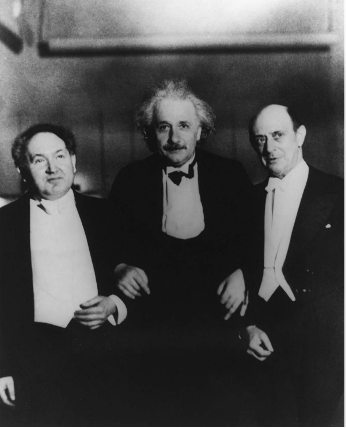
\includegraphics[width=0.8\textwidth]{image/im1.png}
    \caption{1934 年,爱因斯坦和勋伯格在纽约的卡内基音乐厅。}
    \label{fig:einstein_schoenberg}
\end{figure}

为了分析勋伯格及其后继者的音乐,音乐学家们发展出了“音高集合论(Pitch Set Theory)”。音高集合论的核心思想是将音高视为一个集合,称为“音级集合(Pitch-Class Set)”,简称 PC Set\cite{forte_structure_2007}。

我们将十二平均律中的12个音高集合用整数 0 到 11 来表示。通常,C=0
\[
    C=0, C\sharp/D\flat=1, D=2, E\flat=3, E=4, F=5, F\sharp=6, G=7, A\flat=8, A=9, B\flat=10, B=11
\]

据此,一个C大三和弦(C,E,G)可以表示为集合 $\{0, 4, 7\}$。音级集合是无序集,因此 $\{0, 4, 7\}$ 和 $\{4, 7, 0\}$ 是同一个集合,它们都表示C大三和弦。并且在12音级数系统中,12与0是同一个音高,因此对于一个音级数我们将其加上12,其音高是保持不变的,所以$\{4, 7, 0\}$ 和 $\{4, 7, 12\}$相同。

从上面例子也可以看到,对于不同的音高集合,它们在某些情况下可能指向的是同一个和弦,因此我们需要在数学上探究一种形式去进行不同集合之间的比较,这便是音级集合的原型(Prime Form)。 一个音级集合的原型,为了便于比较,其第一个数我们往往令其为0,但更重要的是,原型需要是\textbf{标准序}

\section{结论}

\bibliography{reference.bib}
\bibliographystyle{plain}

\end{document}
